%%%%%%%%%%%%%%%%%%%%%%%%%%%%%%%%%%%%%%%%%%%%%%%%%%%%%%%%%%%%%%%%%%
%%%%%%%% ICML 2012 EXAMPLE LATEX SUBMISSION FILE %%%%%%%%%%%%%%%%%
%%%%%%%%%%%%%%%%%%%%%%%%%%%%%%%%%%%%%%%%%%%%%%%%%%%%%%%%%%%%%%%%%%

% Use the following line _only_ if you're still using LaTeX 2.09.
%\documentstyle[icml2012,epsf,natbib]{article}
% If you rely on Latex2e packages, like most moden people use this:
\documentclass{article}

% For figures
\usepackage{graphicx} % more modern
%\usepackage{epsfig} % less modern
\usepackage{subfigure} 

% For citations
\usepackage{natbib}

% For algorithms
\usepackage{algorithm}
\usepackage{algorithmic}

% As of 2011, we use the hyperref package to produce hyperlinks in the
% resulting PDF.  If this breaks your system, please commend out the
% following usepackage line and replace \usepackage{icml2012} with
% \usepackage[nohyperref]{icml2012} above.
\usepackage{hyperref}

% Packages hyperref and algorithmic misbehave sometimes.  We can fix
% this with the following command.
\newcommand{\theHalgorithm}{\arabic{algorithm}}

% Employ the following version of the ``usepackage'' statement for
% submitting the draft version of the paper for review.  This will set
% the note in the first column to ``Under review.  Do not distribute.''
\usepackage[accepted]{icml2012} 
% Employ this version of the ``usepackage'' statement after the paper has
% been accepted, when creating the final version.  This will set the
% note in the first column to ``Appearing in''
% \usepackage[accepted]{icml2012}

% The \icmltitle you define below is probably too long as a header.
% Therefore, a short form for the running title is supplied here:
\icmltitlerunning{Detecting stress level through computer usage pattern}

\begin{document} 

\twocolumn[
\icmltitle{Detecting stress level through computer usage pattern }

% It is OKAY to include author information, even for blind
% submissions: the style file will automatically remove it for you
% unless you've provided the [accepted] option to the icml2012
% package.
\icmlauthor{name1}{email1}
\icmladdress{school addy}
\icmlauthor{name1}{email1}
\icmladdress{school addy}

% You may provide any keywords that you 
% find helpful for describing your paper; these are used to populate 
% the "keywords" metadata in the PDF but will not be shown in the document
\icmlkeywords{stress, machine learning, computer usage}

\vskip 0.3in
]

\begin{abstract} 
Stress is inevitable. Sometimes people fall back to their old habits or perform a series of actions that can be directly linked to their stressful states. Identifying stress is important but the approach scales poorly when invasive sensors have to be used or the method relies on induced stress in a timed lab experiment.  Our solution aims to identify stressful states based on continuous logging of keystroke dynamics, mouse patterns, and foreground application usage. We propose a privacy-aware system, E-stress detector, that logs participants' computer activities alongside their stress self report. After extracting relevant features, our top classifiers provide 85 to 95 \% accuracy for predicting user future stress level based on historical data. 
\end{abstract} 

\section{Introduction}
\label{introduction}

As we know, overstress undermines our productivity, and more seriously, it might bring harm to our health, even cause mental diseases. However, sometimes we tend to feel exhausted and stressed, but unaware of what cause us to feel stressed exactly. Therefore, it is crucial to find out the sources of stress, and at some appropriate time, give  users some reminders that you are overstressed and you should take a break and relax yourself right away.

When people are under stress, their behaviors tend to change accordingly. In particular, we have observed that people’s computer using patterns, the way they type, click, browse webs change with regard to their stress, or anxiousness level. For example, when people feel stressed, they click the mouses with higher frequency; they tend to have more typos, and thus the frequency of doing error correction raises; the frequency of switching between different web pages also increases; they might check their phones more frequently but unconsciously, etc. We suppose these are good indicators to users’ stress level, and by analyzing users’ baseline stress level and detecting abnormal stress level, we will be able to understand whether they are overstressed and give proper reminders.

Since the computing age has encouraged working on personal computers, stress detection correlated to usage of these electronic devices could lead to insightful results. This research aims to discover which computer activities, if any, correlate with individual stress levels. Can one’s typing pattern, duration on a browser, rate of mouse clicking or overall computer usage be linked to their stress level?  Insightful results could have multiple applications such as personalized health recommendation systems for handling stress, timely interventions for detecting stress at an individual’s peak, holistic feedback for doctors during diagnosis, among other health driven and personal purposes. 

\section{Related Work}
Computer activities such as keystroke dynamics and mouse click patterns have been used in detecting user emotional and stress states. Related works can be broadly grouped into three major categories: Affective Computing, Keystroke Dynamics, and Mouse Usage. 

\subsection{Affective Computing}
Epp Clayton et al, arguably did the first major work connecting keystroke dynamics and emotional states. This research measured 15 emotional states of users using periodical self report and keystroke features throughout the day \cite{epp2011identifying}. Hong proposed StressSense, which can detect human stress by focusing on  paralinguistic features instead of actual vocal contents \cite{lu2012stresssense}. StudentLife utilized SurveyMonkey and mobileEMA to measure participants’ stress as ground truth \cite{wang2014studentlife}. Similarly, we will use the same approach as our ground truth. Instead of 15 emotional states, our research primarily focuses on user's level of stress.

\subsection{Keystroke Dynamics}
Hernandez, Javier, et al in Under Pressure use a pressure sensitive keyboard and capacitive mouse to discriminate between stressful and relaxed states in a lab setting \cite{hernandez2014under}. To allow our application to scale easily, we do not rely on using custom hardware.

\subsection{Mouse Usage}
Early work done by Ark Wendy S. et al in The Emotion Mouse relate the mouse touch to the emotion attached to a computer task. GSR and chest sensors were used to collect heart rate, temperature, galvanic skin response (GSR), and somatic movement, which were measured against the six Ekman’s facial emotions \cite{ark1999emotion}. In more recent work, Sun, David et al in MouStress proposed an approach to detect stress from mouse motion, but from a physiological perspective--- a model of the arm \cite{sun2014moustress}. Our approach is less intrusive as we do not propose an external sensor; rather, we focus on  non-invasive continuous mouse tracking activites such as click rate and coordinates.

\subsection{Computer Applications}
Karpathy on his blog shows how he measures computer activities for self tracking. However, this is done with the idea of quantified self but without linking user stress state. Some of the ideas used in our project design were inspired by work on Karpathy's system \cite{karpathy}.

Our work differs from all other works in 3 major ways: a custom hardware does not need to be installed; data collection is not done in a stress-induced lab setting for a short period of time, rather data is continuously logged with the intent of long-term continuity; as far as we know, we are the first to incorporate computer usage application as part of stress sensing. 

Unlike previous works, which focus on only keystrokes, only mouse, or both, our work leverages foreground application usage as an extra data source. This is based on the intuition that certain applications might immensely affect user emotional state compared to others. For instance, a non-programmer using Matlab for the first few days might hit the backspace key to delete wrongly written code; click on the menu buttons several times, perhaps in search of a functionality or switch applications multiple times between Matlab software and a browser page showing ``how to perform matrix multipication in Matlab''.

It is worthwile to note that previous works have logged user computer activities without explicitly discussing how user data is protected; our application takes a different approach by only logging specific keys when users type. Every other key is blocked with the symbol ``\$\$''. For instance, alphabetic and numeric keys are logged as ``\$\$'' as a user could type highly sensitive information such as passwords or personal messages. In addition, every data logged is not uploaded to a cloud server; the data is locally stored on the user's computer. This way, a user can decide to opt out of the data logging process and delete all data collected.

\section{Methodology}
The work involves two major components: the data logging process done in-situ -- as participants carried out their daily activities, and the data processing required to classify stress states. For the data collection, users' keystrokes, mouse activities, and computer applications usage are timestamped and logged. The data processing involved extracting relevant keystroke features in order to build Machine Learning classifiers. 

\subsection{Experience Sampling of Computer Activities}
Experience Samping Method (ESM) involves continuously logging computer activities while periodically collecting user responses to self-reports of their level of stress \cite{hektner2007experience}. Stress states were measured using Photographic Affect Meter (PAM) \cite{pollak2011pam}and three-question likert-scale survey. 

Figure \ref{pam} shows the PAM survey. During periodic interval---we arbitrarily select 30 minutes interval---a webpage automatically opens up and a user is asked \textit{``How do you feel right now?''} Then the user selects one of 16 grid pictures that reflects their internal emotional state. 

Figure \ref{ema} shows a self-report questionnaire. After selecting a picture in PAM, a 3-question survey page opens up where the user gets to pick one response out of five categories. 

\begin{figure}[ht]
		\centering
		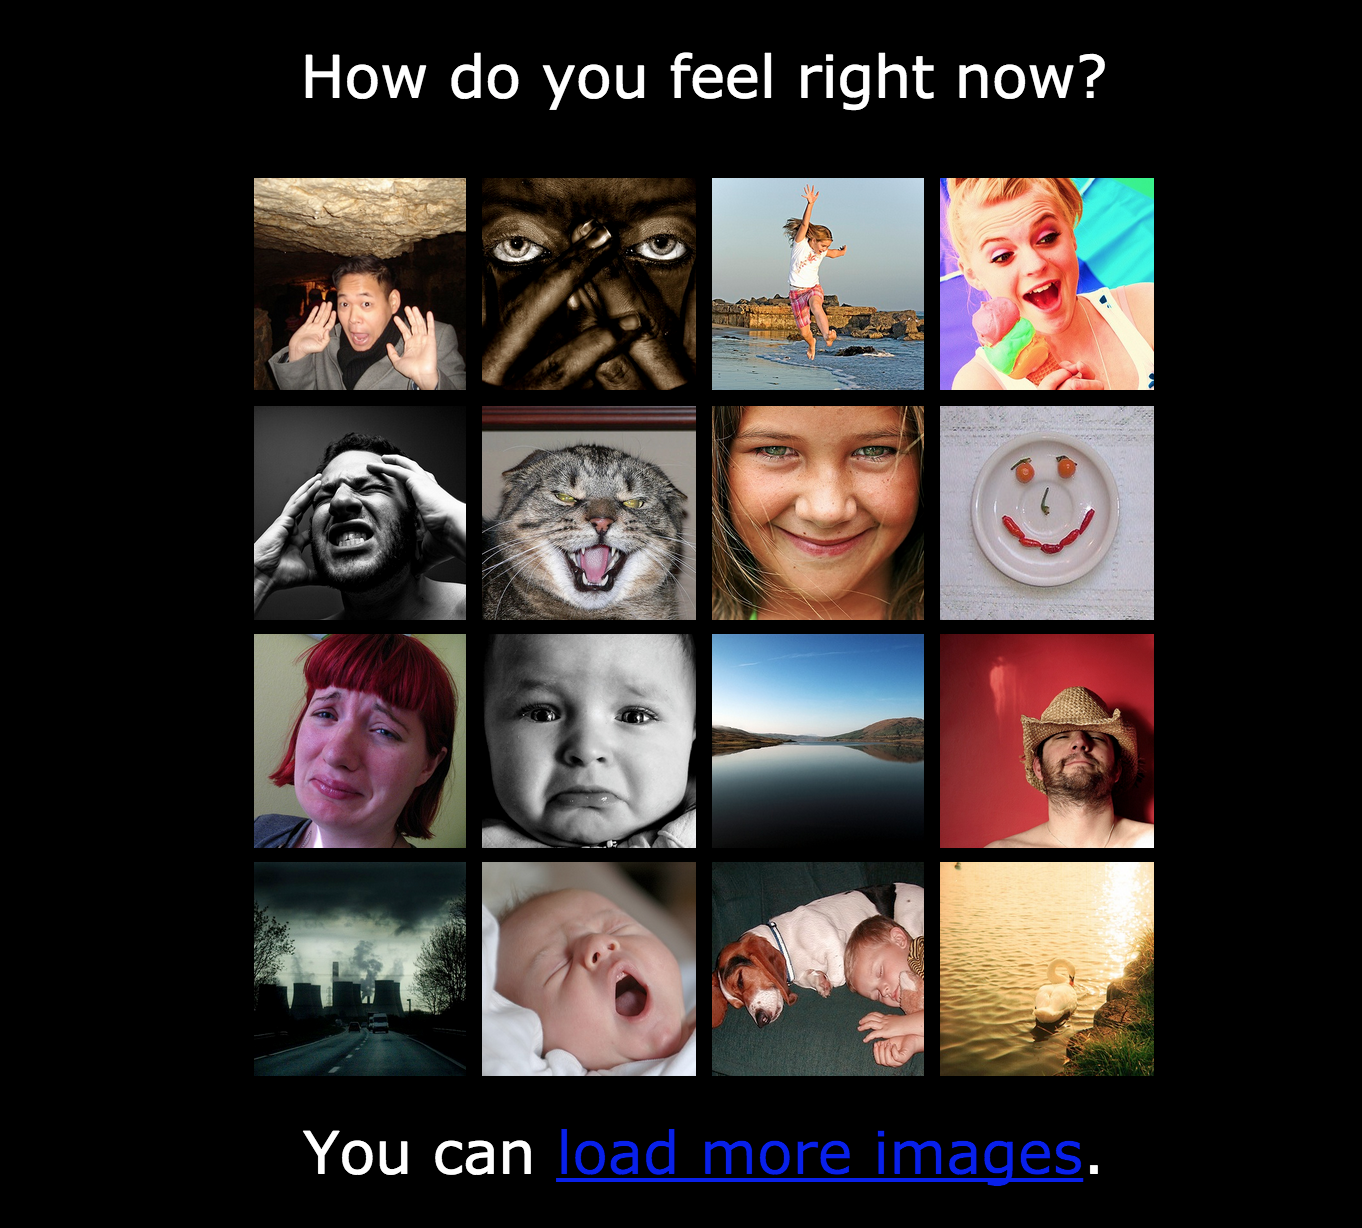
\includegraphics[width=\columnwidth]{pam}
		\label{pam}
		\caption{PAM: the user selects one of 16 grid pictures that reflects their internal emotional state.} 
		\label{pam}
\end{figure} 




\begin{figure}[ht]
	\vskip 0.2in
	\begin{center}
		\centerline{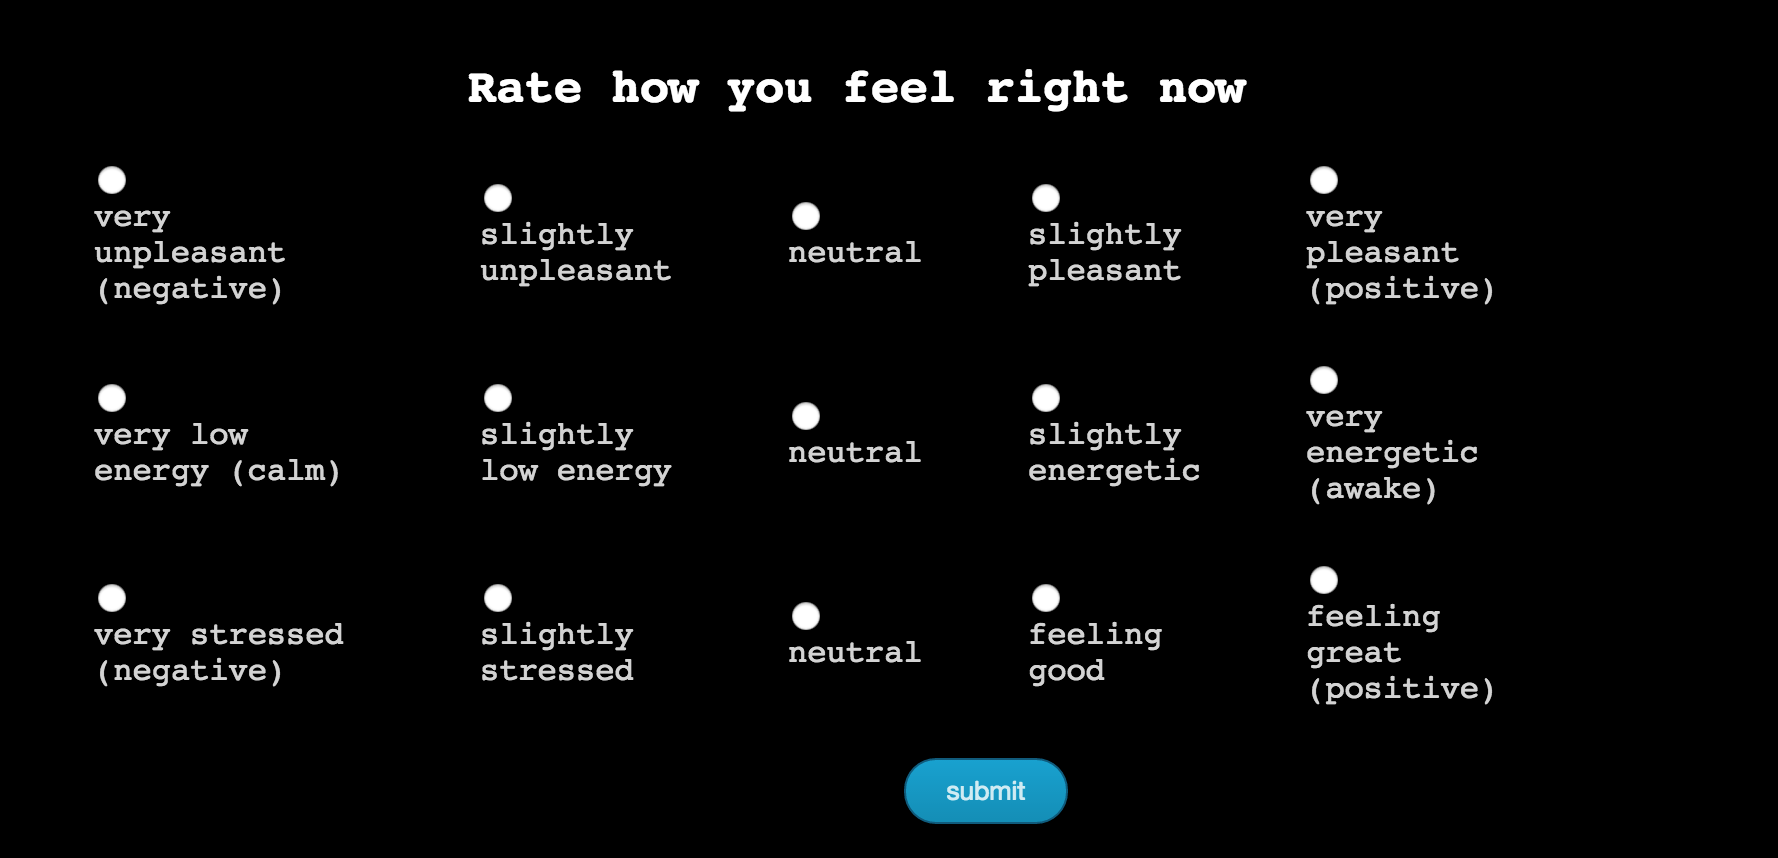
\includegraphics[width=\columnwidth]{ema}}
		\caption{A 3-question survey: the user gets to pick one response out of five categories for each question. 
		}
		\label{ema}
	\end{center}
	\vskip -0.2in
\end{figure} 


\subsection{Data Collection Software}
A system was built that logs user keystrokes, mouse activities and applications used throughout the day. While there are a few open sourced tools that could have been adopted, a custom application was built because existing tools suffer from poor documentation and incomprehensible programming approaches. 

Upon installation, our software tool contains a keystroke logger, a mouse logger, an application logger and a self-report logger. The keyboard and mouse applications continuously logs keystrokes and mouse activities; the foreground application is logged every 3 seconds; while the stress self-report is logged every 30 minutes. The self-report application starts up a PHP server, opens PAM webpage with the user's default browser. Upon selecting a choice from the 16-grid pictures, the response is saved in a file. Thereafter, the 3-question survey is opened as the next webpage, which upon answering a ``thank-you'' page loads. After about 5 seconds, the ``thank-you'' page automatically closes. Self-report application logs user response based on when they responded and not when the page opens. For instance, if the Web page opens at 4pm but the user responds at 7pm, then the response is logged at 7pm. 

Every 15 minutes, a background script checks if all the applications are running or if they have been stopped either manually by the user, another running process, or through a power down of the user computer. This ensures that user logging continues non-intrusively as users do not have to manually start the applications if they were shut down. In order to maintain user access control, every activity application has an icon that appears in the dock so that the user can close the application whenever they want to; users can also delete the data directory if they don't want to partake in the experiment. These intervals for each application were arbitrarily chosen. 

mouse logging format
2015-05-03 12:18:55.438360 |      MouseMoveHooker |           NSMouseMoved | y=606.19140625 x=683.0390625
2015-05-03 12:19:51.473070 |    MouseButtonHooker |         NSRightMouseUp | y=22.234375 x=274.37109375
2015-05-03 12:19:55.261508 |    MouseButtonHooker |          NSLeftMouseUp | y=272.79296875 x=293.51953125
2015-05-03 12:19:53.588968 |    MouseButtonHooker |        NSLeftMouseDown | y=81.90234375 x=109.9609375


keyboard logging format
%2015-05-03 12:18:57.540228 |            KeyHooker |                NSKeyUp | char=  mods=[] key=49 is_repeat=False
%2015-05-03 12:20:28.903225 |            KeyHooker |              NSKeyDown | char=\$\$ mods=['COMMAND'] key=\$\$ is_repeat=False


application logging format
%2015-05-07 22:39:09.113787 |        Google Chrome


pam logging format
%time: 2015-04-29 23:47:11, image_id: 11, cell_id: 4, pam_pa: 16, pam_na: 3, arousal: 4, valence: 4

ema logging format
%time: 2015-04-27 03:59:49, pleasant_state: slightly_pleasant, energy_state: slightly_energetic, stress_state: feeling_good

 
Using our custom applications, we will install our background scripts on the participants’ computers. Ideally, our background programs will record the keys users type, but the corresponding values will be randomized due to privacy sensitivity, and the frequency of mouse clicking as well.
Data for Web browsing and application usage will be collected through available python APIs. All the data will be stored as text files awaiting further analysis.

\subsection{Feature Extraction}
We segmented the raw computer usage activities with sliding window size = 1 minute and the extracted three types of computer usage features, \textbf{M}, \textbf{K}, and \textbf{A} for mouse clicks, keystrokes, and application usage within each sliding window. \textbf{M} = $[d_{m}, r_{m}, t_{m}]$, where $d_{m}$ is the total distance of mouse movement, $r_{m}$ is the mouse click rate, and $t_{m}$ is the average mouse button pressed duration. \textbf{K} = $[r_{k_1}, t_{k_1}, r_{k_2}, t_{k_2}, t_{k_i}, ..., r_{k_N}, t_{k_N}]$, i $\in{N}$, where $k_{i}$ stands for different keys and N stands for total number of key types we logged, and $N=9$ in our case, including function keys, letter keys, enter key, tab key, space key, delete key, escape key, arrow key, and all the keys that were pressed (that is, the previous key types were also taken into account), and $t_{k_i}$ is key pressed time for key $k_{i}$.  \textbf{A} = $[t_{a_1}, t_{a_2}, t_{a_j}, ..., t_{a_P}, x]$, j $\in{P}$, where $a_{i}$ stands for different applications, $P$ is the total number of applications users might open when using computers, $t_{a_j}$ is the time users spent on application $a_{j}$, and $x$ is the number of active applications within each time window. To know decide what $P$ is, we first iterated through the users' historical application usage logs.

\subsection{Algorithm}
Since the self-report survey popped up every 30 minutes, we only considered raw computer usage features within the 30-minute duration, if the computer was active,  before the survey is filled out. That is, assuming the user filled out the survey at timestamp $T_end$, and the computer got active at timestamp $T_c$, we only considered raw features with timestamps in $[T_{begin}, T_s)$, where $T_{begin}$=$min(T_{end-1800}, T_c)$. Then according to the previous section, we extracted high level features from the raw features among each period and got computer usage samples $S_{T_{begin}}, S_{T_{begin+60}}, ..., S_{T_{end-60}}, S_{T_{end}}$, where each sample $S$ was labeled with the corresponding binary results of users' stress level based on the participants' EMA self-report score. 

Due to time limit, we could only collect data from one participant for consecutive 3 days after the deployment, and we got 352 samples from the deployment. We used Decision Tree, Random Forest and support vector machine (SVM) for stress prediction. We tried  different ways of splits for training and testing, from 50-50 split to 90-10 split. Figure \ref{prediction} is the accuracy of stress prediction with different algorithms as well as different ways of data splits. For the baseline algorithm, it randomly guesses whether the user is stressed or not.

\begin{figure}
	\centering
	\begin{subfigure}
		\centering
		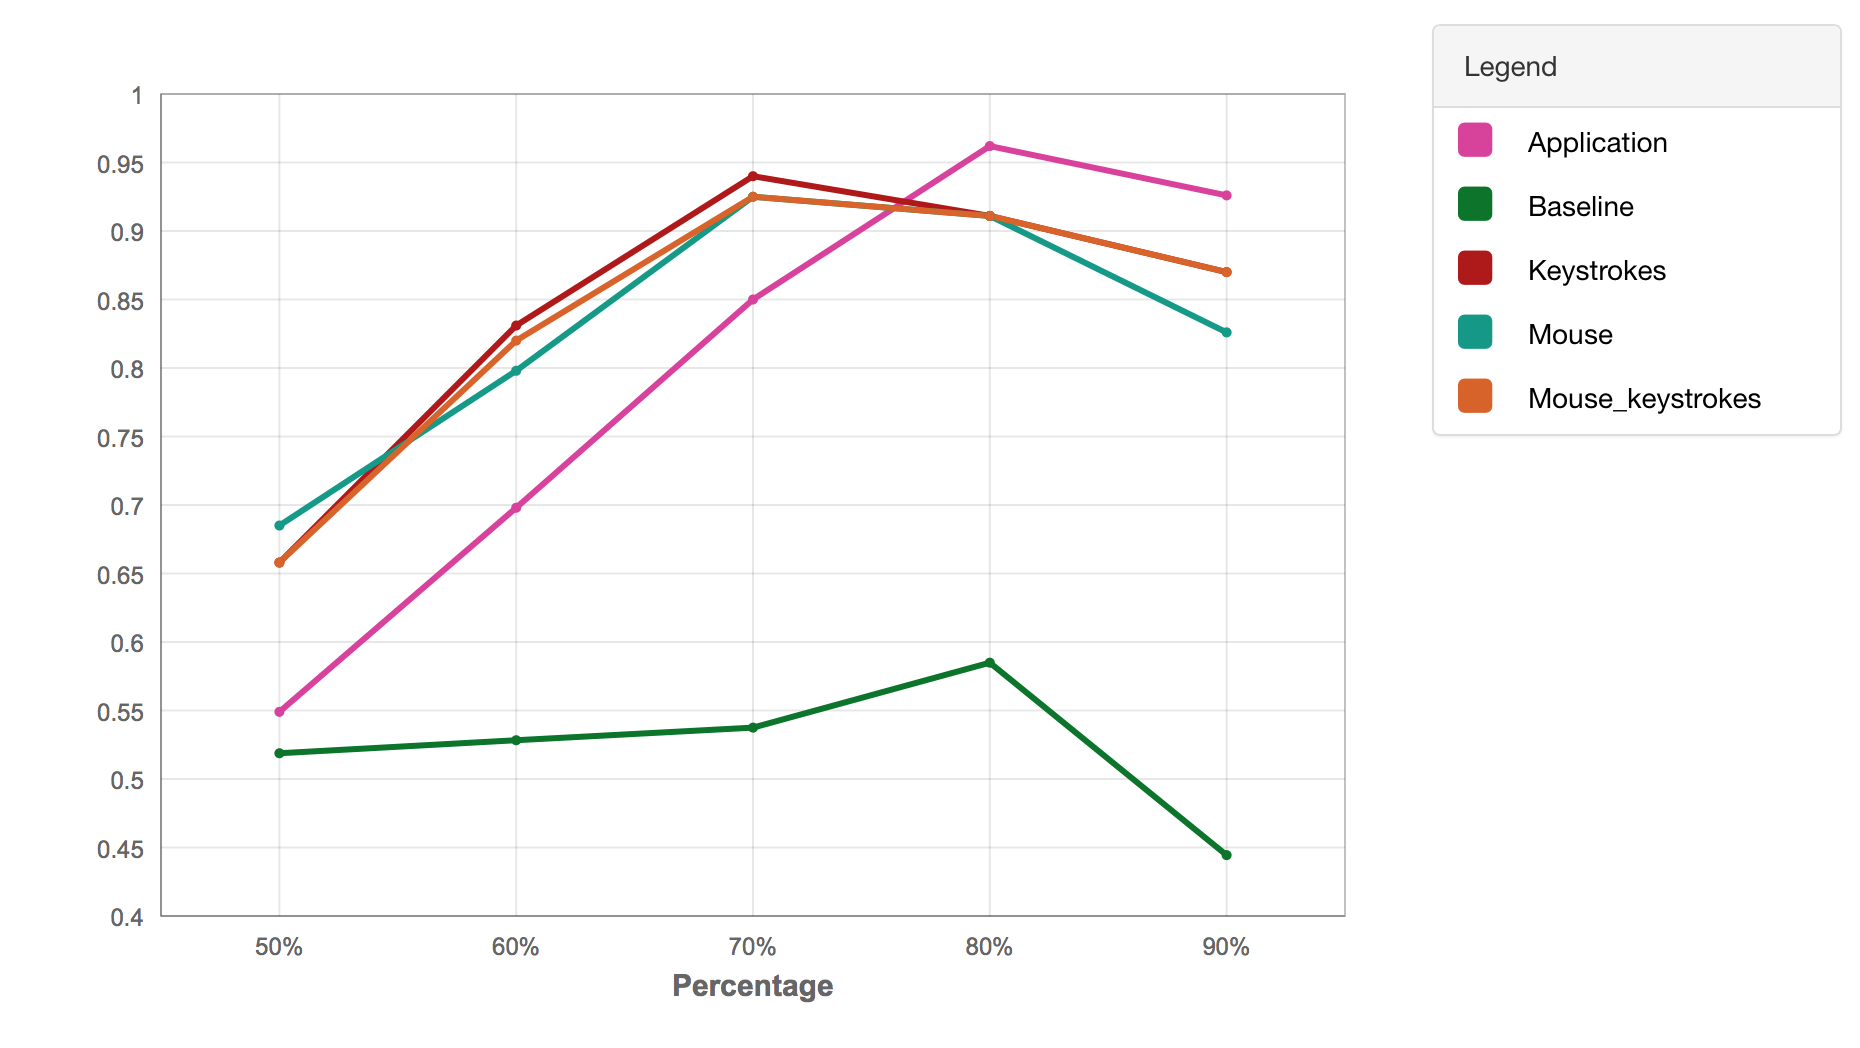
\includegraphics[width=\columnwidth]{DecisionTree.png} {a. Decision Tree}
	\end{subfigure}
	\begin{subfigure}
		\centering
		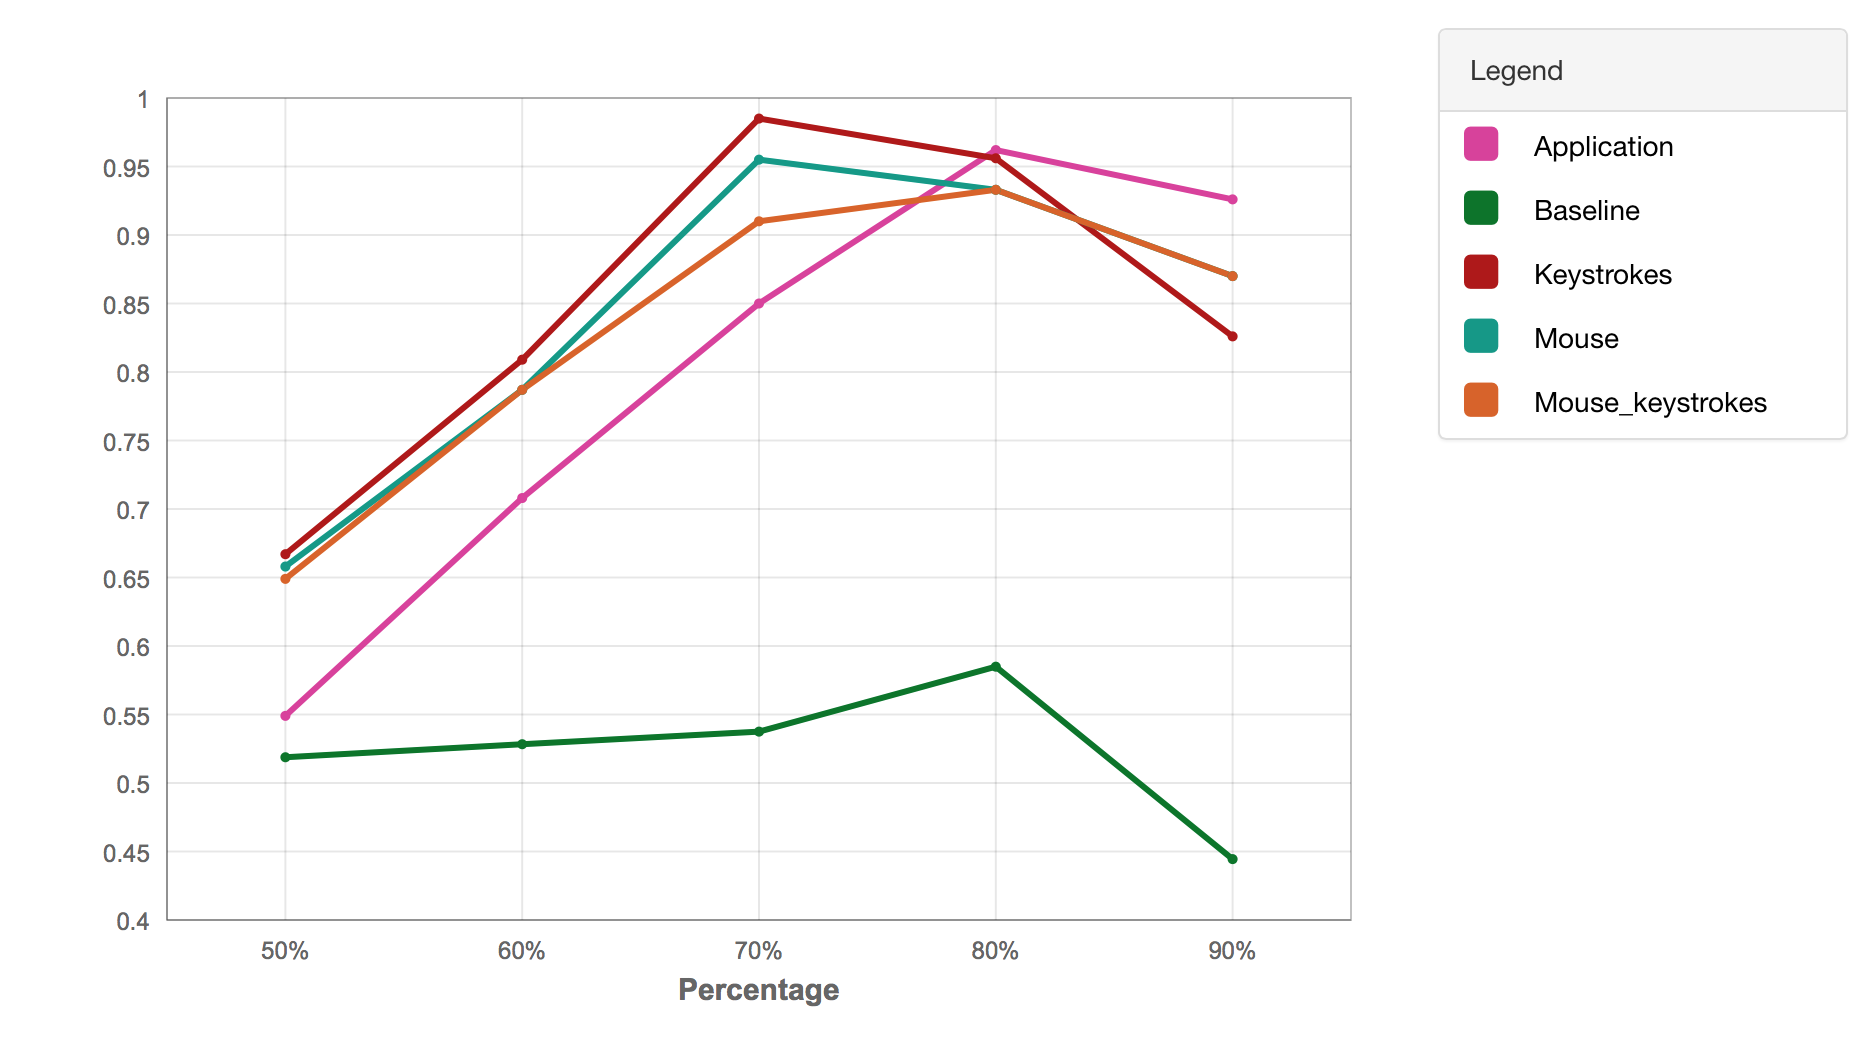
\includegraphics[width=\columnwidth]{RandomForest.png} {b. Random Forest}
	\end{subfigure}
	\begin{subfigure}
		\centering
		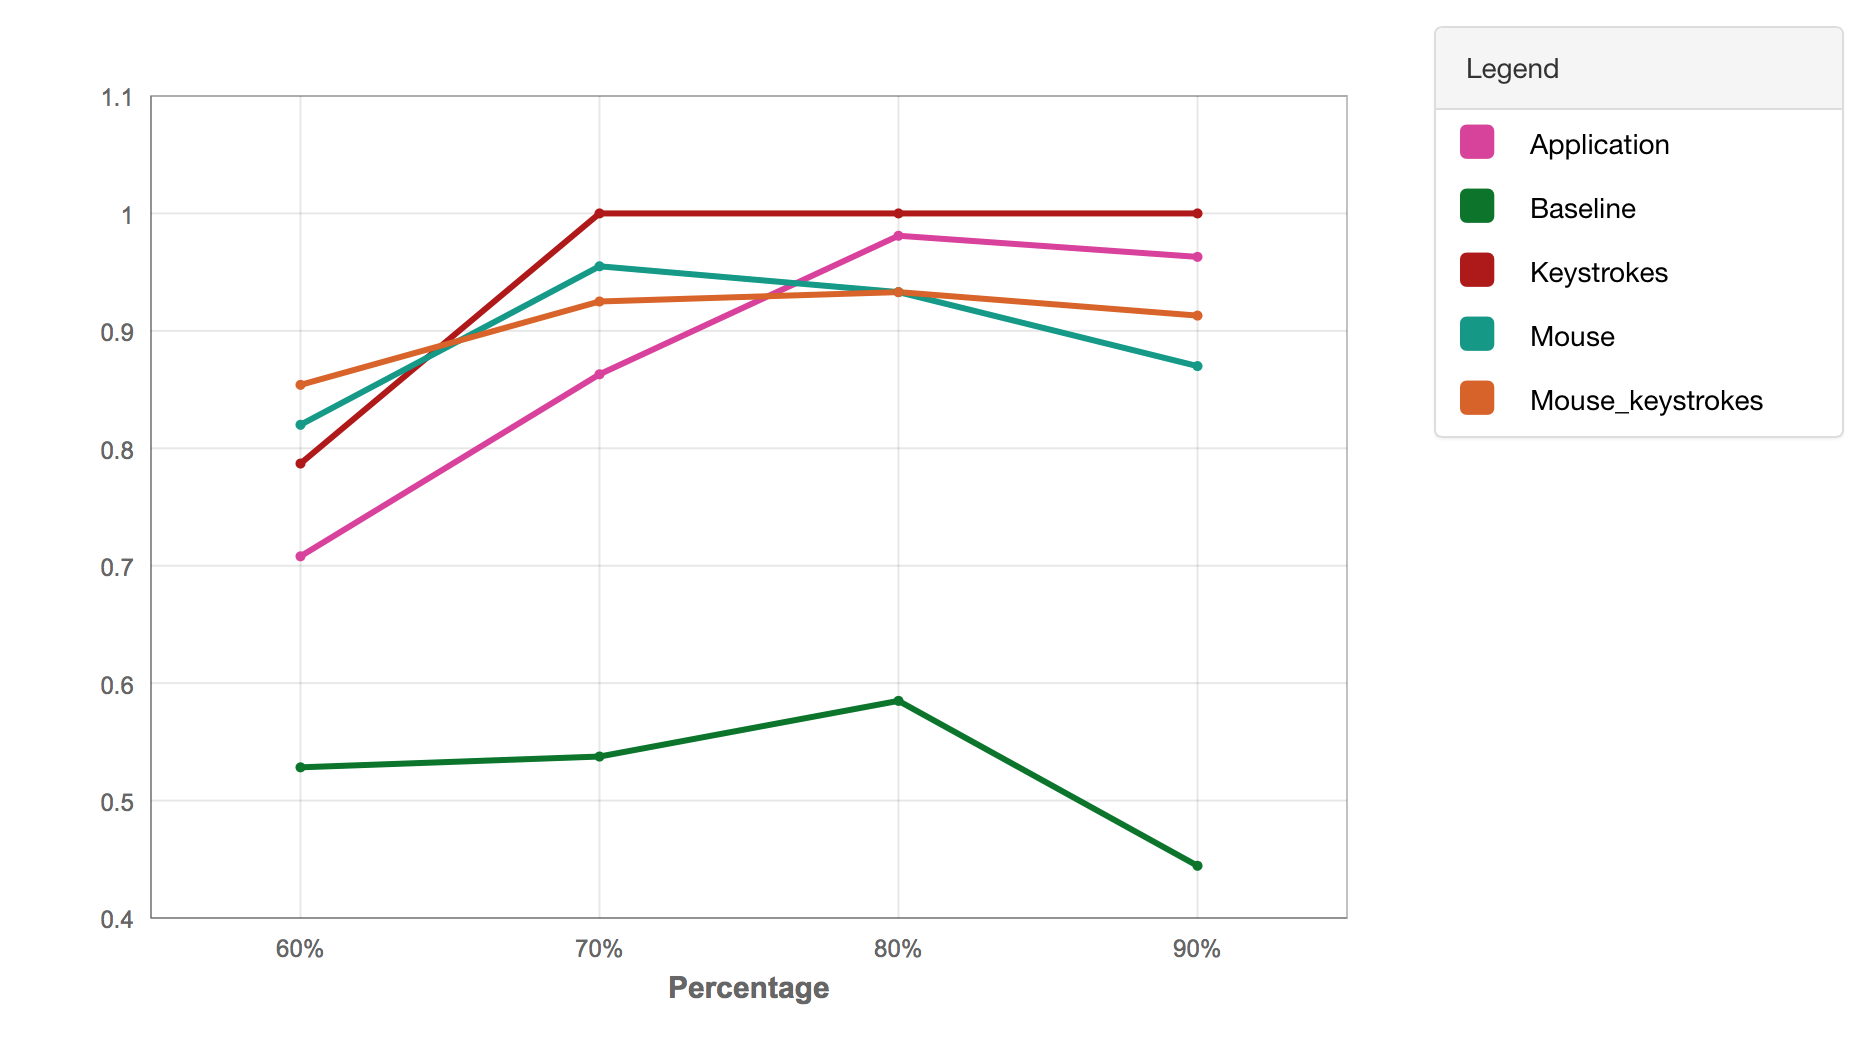
\includegraphics[width=\columnwidth]{SVM.png} {c. SVM}
	\end{subfigure}
	\caption{The accuracy of stress prediction with different algorithms: (a) Decision Tree, (b) Random Forest, (c) Support Vector Machine (SVM) and with different ways of data splits.} \label{prediction}
\end{figure}

\begin{figure}[ht]
	\vskip 0.2in
	\begin{center}
		\centerline{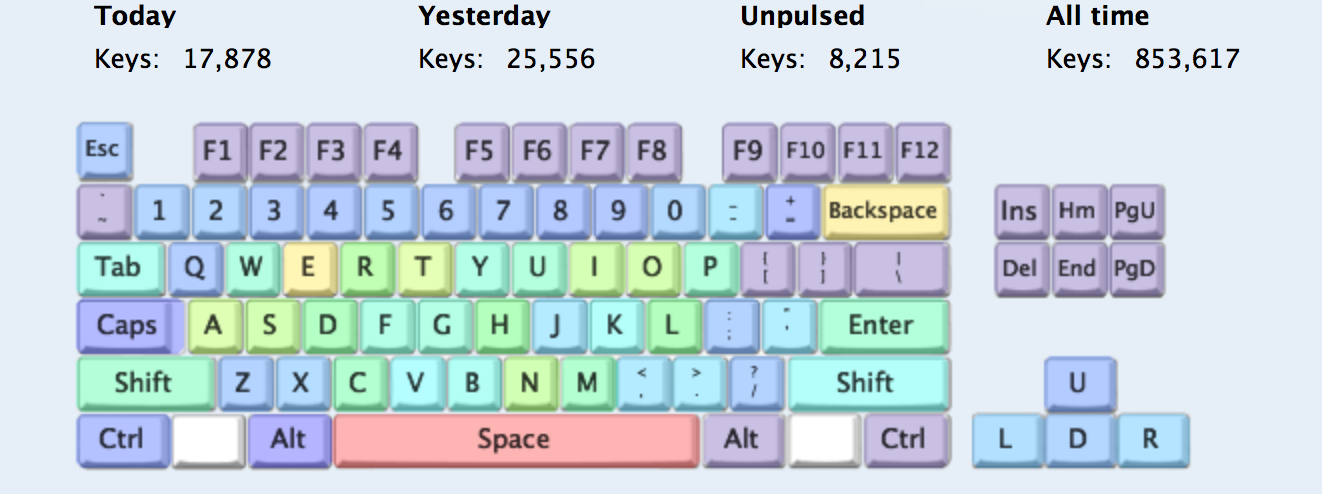
\includegraphics[width=\columnwidth]{keyboard}}
		\label{keyboard}
		\caption{Keyboard Heatmap}

		\label{icml-historical}
	\end{center}
	\vskip -0.2in
\end{figure} 

\begin{figure}[ht]
	\vskip 0.2in
	\begin{center}
		\centerline{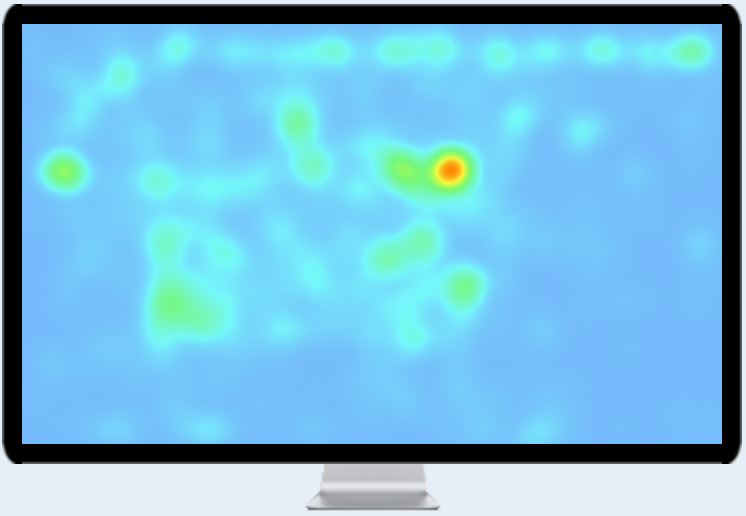
\includegraphics[width=\columnwidth]{mouse_movement}}
		\caption{Mouse Keystrokes
		}
		\label{icml-historical}
	\end{center}
	\vskip -0.2in
\end{figure} 

\section{Discussion}
coming soon from Vincent


\subsection{Limitations}
Our dataset is limited. Since recruited participants were PhD students, our prediction model performance cannot be generalized to a broader audience. Since self-report surveys are subject, the definition of stress for different participants will have varying likert scale values. 

Survey popping up periodically can become annoying to users thereby making reducing performance over time. Since emotional states are short-lived and a user can have multiple emotions in a short time, the surveys cannot fully capture the end user's entire emotional states but only a fraction of it



\section{Future Work}
In order to improve multimodal sensing, future work will involve external sensors for measuring HR, BP, EEG. The current application focuses on batch learning of data already amassed so for next iteration will involve online learning especially for making efficient recommendation systems. Participants for this experiment were PhD students recruited from a research lab familiar with some of the measuring tools used; more insightful applications might involve workers in industries especially end users oblivious of the methods of the current research.

do some form of active learning

collect data for a longer period of time --- like several months


\subsection{Conclusion}

% Acknowledgements should only appear in the accepted version. 
\section*{Acknowledgments} 
Special thanks to Prof Daniel Cosley, students of INFO 6010, reviewers of Advanced Machine Learning course (Spring 2015), members of the PAC lab at Cornell University Information Science, and Prof Tanzeem Choudhury, whose guidance was instrumental in this project. 

% In the unusual situation where you want a paper to appear in the
% references without citing it in the main text, use \nocite

\bibliography{ml_paper}
\bibliographystyle{icml2012}

\end{document} 


% This document was modified from the file originally made available by
% Pat Langley and Andrea Danyluk for ICML-2K. This version was
% created by Lise Getoor and Tobias Scheffer, it was slightly modified  
% from the 2010 version by Thorsten Joachims & Johannes Fuernkranz, 
% slightly modified from the 2009 version by Kiri Wagstaff and 
% Sam Roweis's 2008 version, which is slightly modified from 
% Prasad Tadepalli's 2007 version which is a lightly 
% changed version of the previous year's version by Andrew Moore, 
% which was in turn edited from those of Kristian Kersting and 
% Codrina Lauth. Alex Smola contributed to the algorithmic style files.  


